\chapter{Wstęp}
\section{Wprowadzenie}
Rola automatyzacji w obsłudze klienta znacznie wzrosła w ostatnich latach. Można to zaobserwować w dynamice, z jaką rozwijane się różne rodzaju serwisy dostępne on-line, łączące dostarczycieli usług czy też sprzedawców z użytkownikami korzystającymi z ich oferty. Szczególnym przypadkiem takich systemów są elektroniczne biura obsługi klienta (eBOK). Takie systemy są szeroko stosowane w różnych branżach sektora usług, takich jak energetyka, wodociągi, telekomunikacja, usługi multimedialne i zarządzanie wspólnotami mieszkaniowymi.

Z punktu widzenia użytkowników główną zaletą eBOKów jest możliwość korzystania z~ich funkcji w dowolnym miejscu i czasie. Cecha ta nie tylko poprawia jakość obsługi klienta, ale także zwiększa efektywność działania instytucji wdrażających takie rozwiązanie. Poza zapewnieniem dostępu do informacji o rozliczeniach i płatnościach, eBOKi wspierają także realizację bardziej zaawansowanych procesów, jak zgłaszanie problemów technicznych, zarządzanie zgłoszeniami serwisowymi i komunikację z zarządem. Ważnym aspektem tych systemów jest bezpieczeństwo danych. Jest ono zapewniane dzięki regularnym aktualizacjom oprogramowania, wdrażaniu mechanizmów uwierzytelniania dwuskładnikowego itp. Powstające systemy muszą być zgodne z przepisami regulującymi sposób ochrony danych osobowych, takimi jak RODO.

Obecnie na rynku spotkać można wiele systemów typu eBOK. Jednym z nich jest system ,,Energa24''. Umożliwia on klientom dostęp do informacji o zużyciu energii, przeglądanie i pobieranie rachunków, dokonywanie płatności online oraz zgłaszanie awarii~\cite{energa}. Standardowy scenariusz dokonywania płatności za pomocą tej aplikacji pokazano na rysunku~\ref{fig:energa_manual}. Użytkownik może wybrać odpowiedni rachunek, a następnie, poprzez bezpieczną bramkę płatniczą uiścić należności bezpośrednio w systemie.
\begin{figure}[htb]
	\centering
		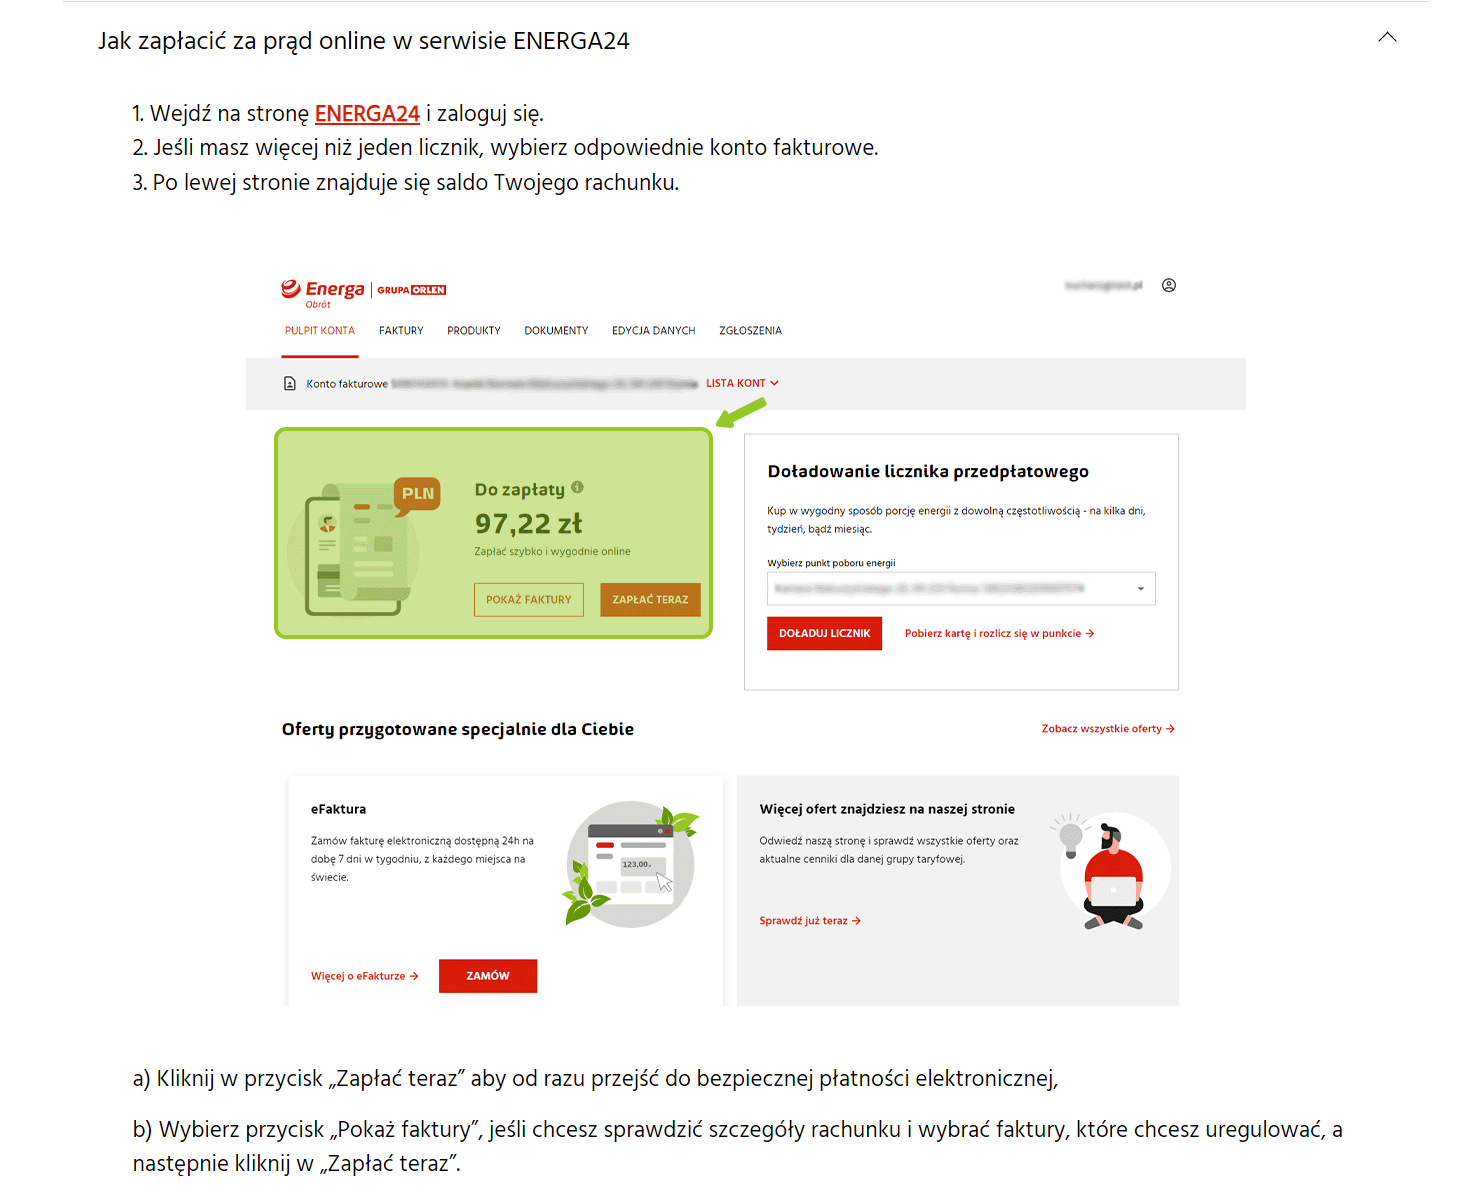
\includegraphics[width=0.91\linewidth]{rys01/energa_manual_1.png} \\[-1ex]
		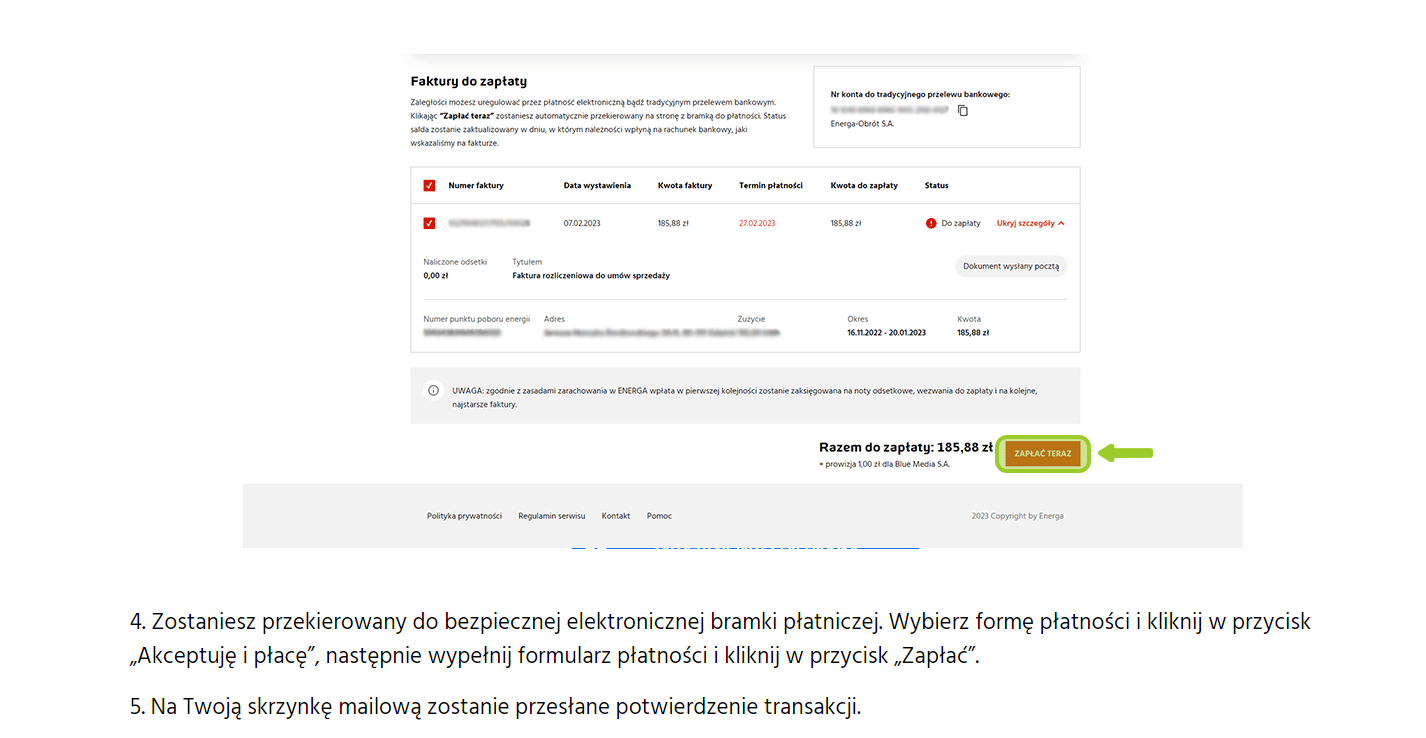
\includegraphics[width=0.91\linewidth]{rys01/energa_manual_2.png} \\[-1ex]
		\caption{Opis scenariusza dokonania płatności za energię elektryczną w serwisie ,,Energa24''~\cite{energa}}
	\label{fig:energa_manual}
\end{figure}

Innym przykładem jest aplikacja ,,Play24'' (choć może lepiej powiedzieć ,,system informatyczny'', względem którego wymieniona aplikacja pełni rolę punktu dostępowego z przyjaznym interfejsem użytkownika), dostarczana przez operatora telekomunikacji Play. Umożliwia ona użytkownikom zarządzanie wykupionymi usługami telekomunikacyjnymi oraz multimediami. Lista funkcji oferowanych przez tę aplikację jest szeroka. Obejmuje, m.in, monitorowanie wykorzystania pakietów internetowych, minut rozmów czy SMS-ów, co pozwala użytkownikom na bieżąco śledzić stan konta i w razie potrzeby dokupować dodatkowe usługi. Użytkownicy mogą również sprawdzać historię swoich aktywności, w tym szczegółowe informacje na temat wysyłanych wiadomości, połączeń czy zakupionych pakietów ~\cite{Play24}.
Na rysunku \ref{fig:play24_manual} 
pokazano przykładowe widoki interfejsu użytkownika, eksponującego funkcje, dzięki którym użytkownicy mogą śledzić swoje zużycie internetu, zarządzać opłatami oraz kontrolować ustawienia sieci domowej.
\begin{figure}[ht]
    \centering
    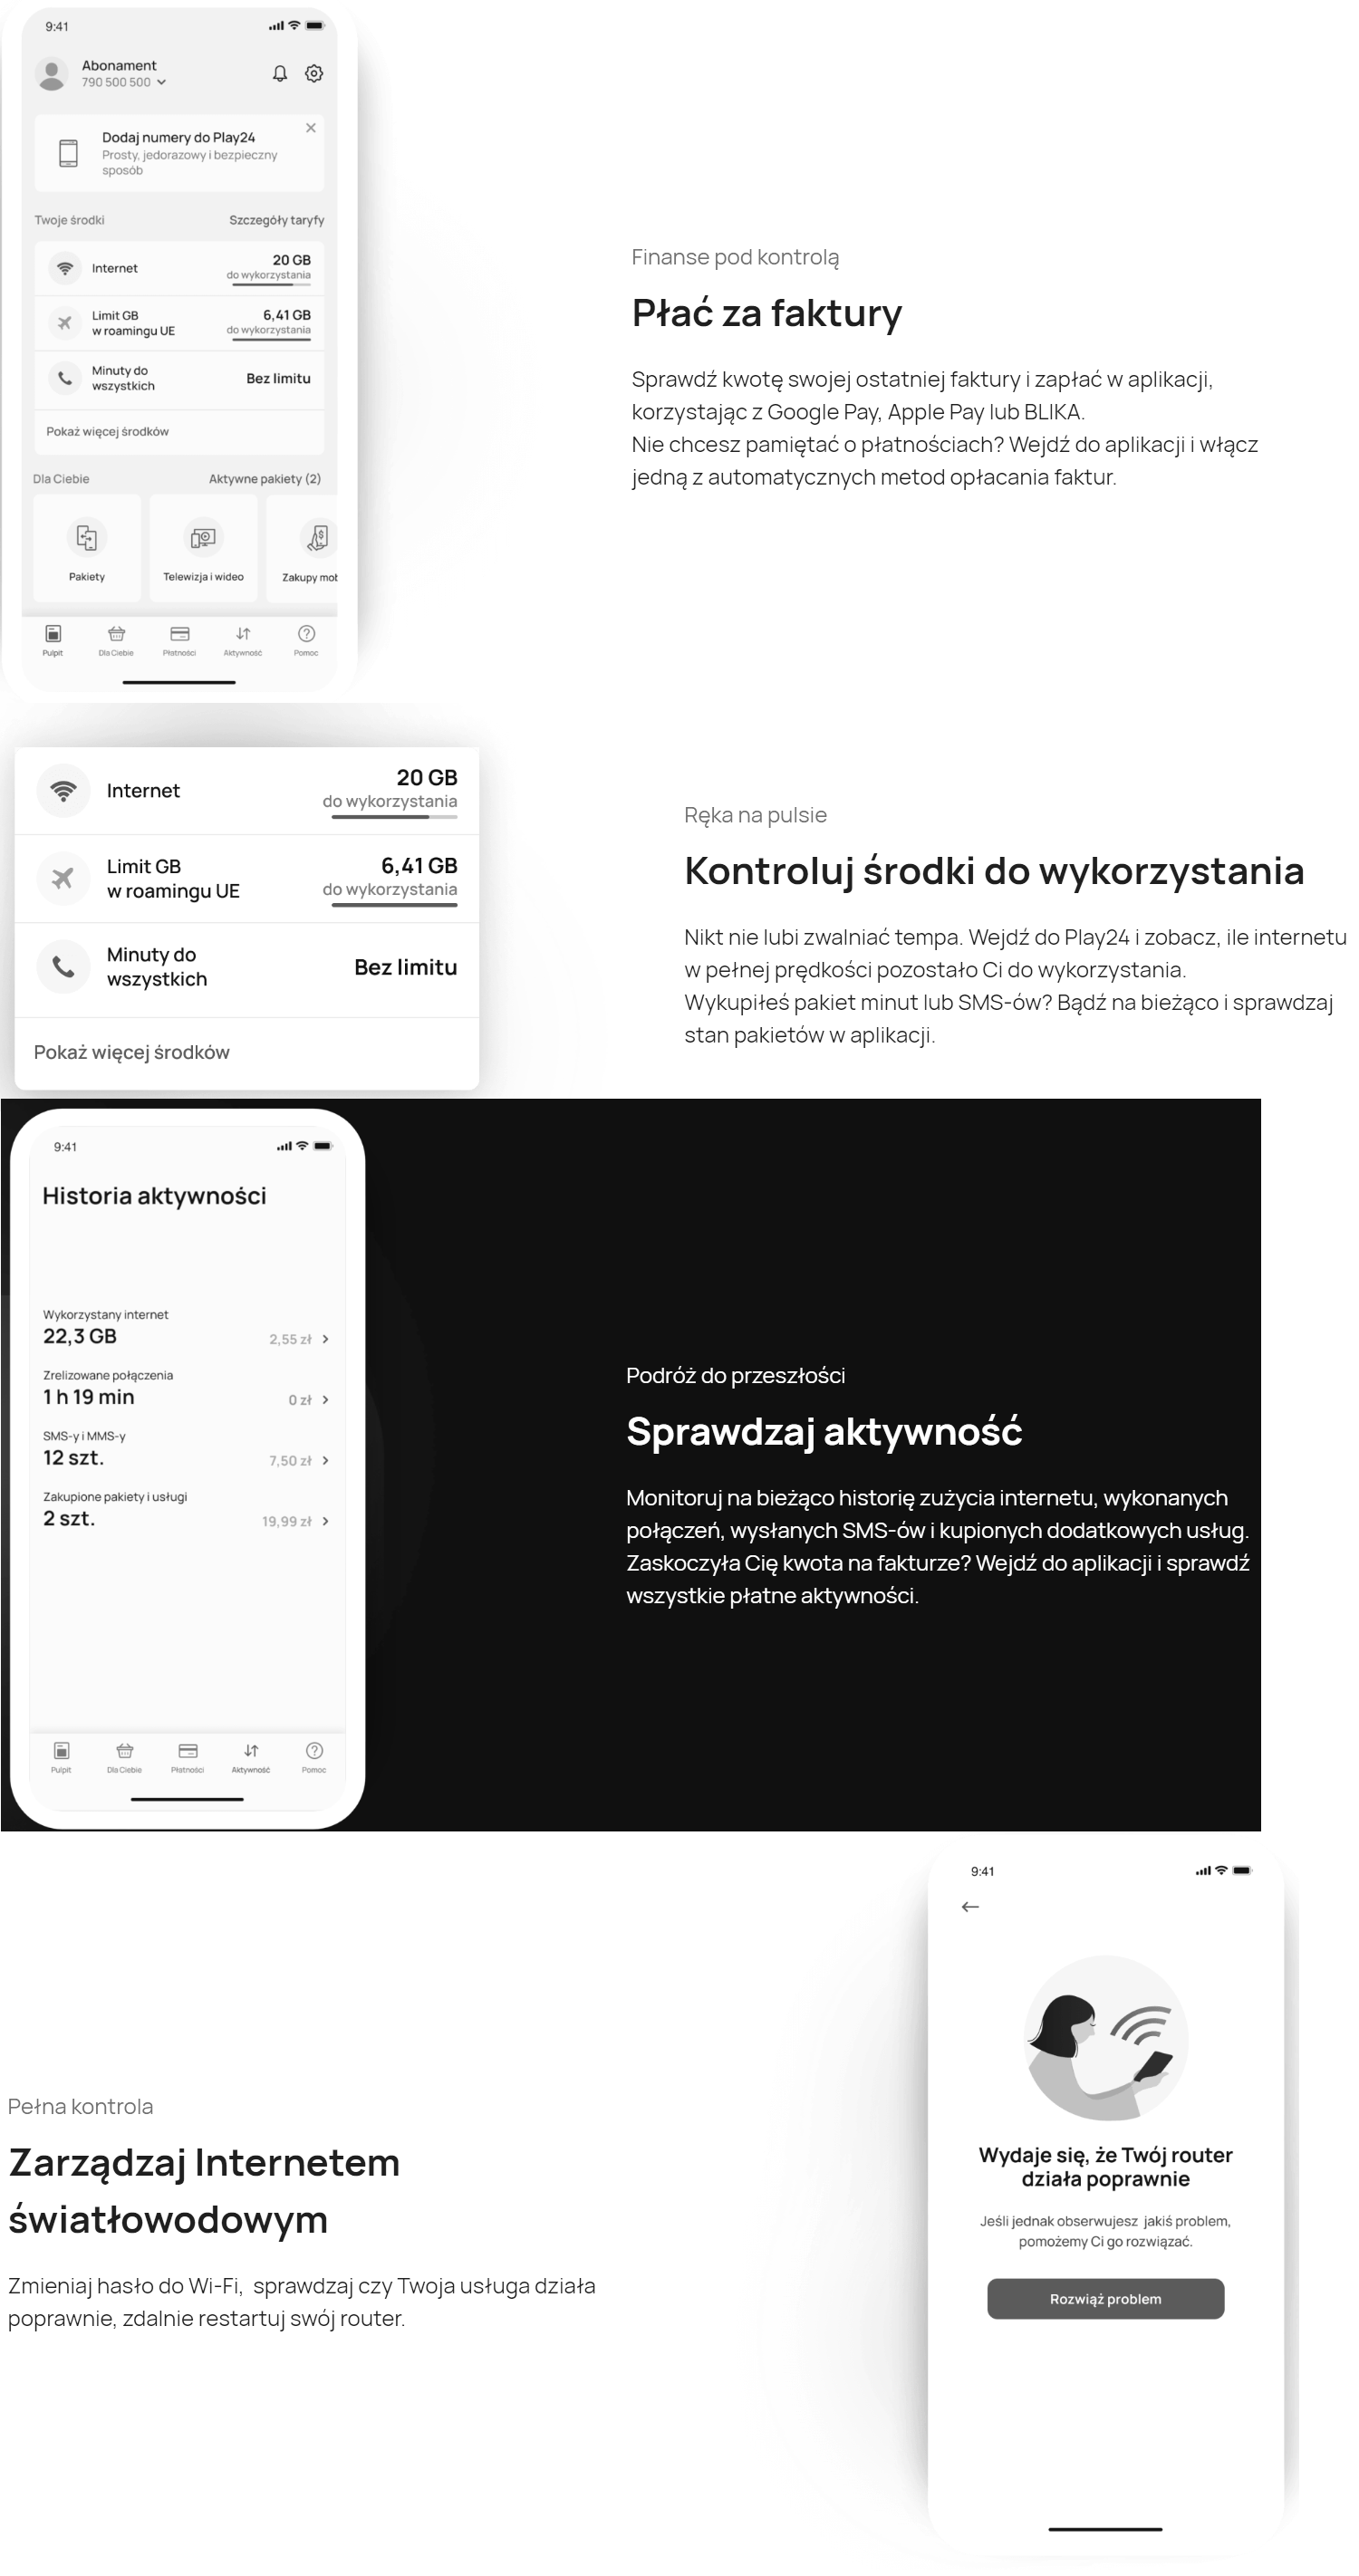
\includegraphics[width=0.63\linewidth]{rys01/play_manual}
    \caption{Opis głównych funkcji oferowanych w systemie ,,Play24''}
    \label{fig:play24_manual}
\end{figure}

Regulowanie płatności może odbywać się różnymi metodami, w tym z wykorzystaniem Google Pay, Apple Pay oraz BLIK. Użytkownicy mogą skonfigurować automatyczne płatności, co znacząco upraszcza zarządzanie opłatami. Dodatkowo, aplikacja umożliwia dostęp do szczegółowych faktur oraz wyciągów z historii transakcji, co pomaga kontrolować bieżące wydatki. Udostępniane panele umożliwiają zarządzanie usługami światłowodowymi, w~tym zdalne restartowanie routera czy zmianę hasła do Wi-Fi. W przypadku problemów technicznych, użytkownicy mogą zgłaszać usterki i diagnozować problemy bezpośrednio z poziomu aplikacji. Dzięki intuicyjnemu interfejsowi, użytkownicy mogą szybko przemieszczać się między funkcjami aplikacji, co znacząco usprawnia zarządzanie usługami telekomunikacyjnymi i~technicznymi.

Na rynku dostępne są również systemy dostosowane specjalnie do potrzeb spółdzielni i wspólnot mieszkaniowych. Przykładem może być system ,,e-Kartoteka'', który umożliwia mieszkańcom zarządzanie zgłoszeniami usterek z podglądem postępu ich obsługi, wgląd oraz regulację w płatności za nieruchomość, wgląd w dokumenty nieruchomości oraz wspólnoty, głosowanie nad uchwałami wspólnoty, a także komunikację z zarządem~\cite{e-kartoteka}. System ten oferuje również możliwość przeglądania rozliczeń mediów, takich jak woda, energia elektryczna czy ogrzewanie, co ułatwia mieszkańcom śledzenie swoich bieżących opłat i zużycia. 

Aplikacja ,,e-Kartoteka'' zapewnia szybki dostęp do wyciągów z rachunków i opłat miesięcznych, w tym szczegółowych rozliczeń za media (patrz rysunek~\ref{fig:kartoteka_manual}). Dzięki intuicyjnemu interfejsowi użytkownicy mogą sprawnie poruszać się między funkcjami rozmieszczonymi na takich komponentach, jak tablica ogłoszeń, forum dyskusyjne dla mieszkańców czy dokumentacja nieruchomości, co znacząco poprawia komunikację i współpracę w obrębie wspólnoty. Ponadto mają oni możliwość zgłaszania odczytów liczników, co automatycznie generuje informacje na temat aktualnego stanu rozliczeń oraz zaległych opłat, podobnie jak widoczne na przedstawionym obrazie funkcje raportowania stanu liczników i przeglądania historii faktur.
\begin{figure}[ht]
    \centering
    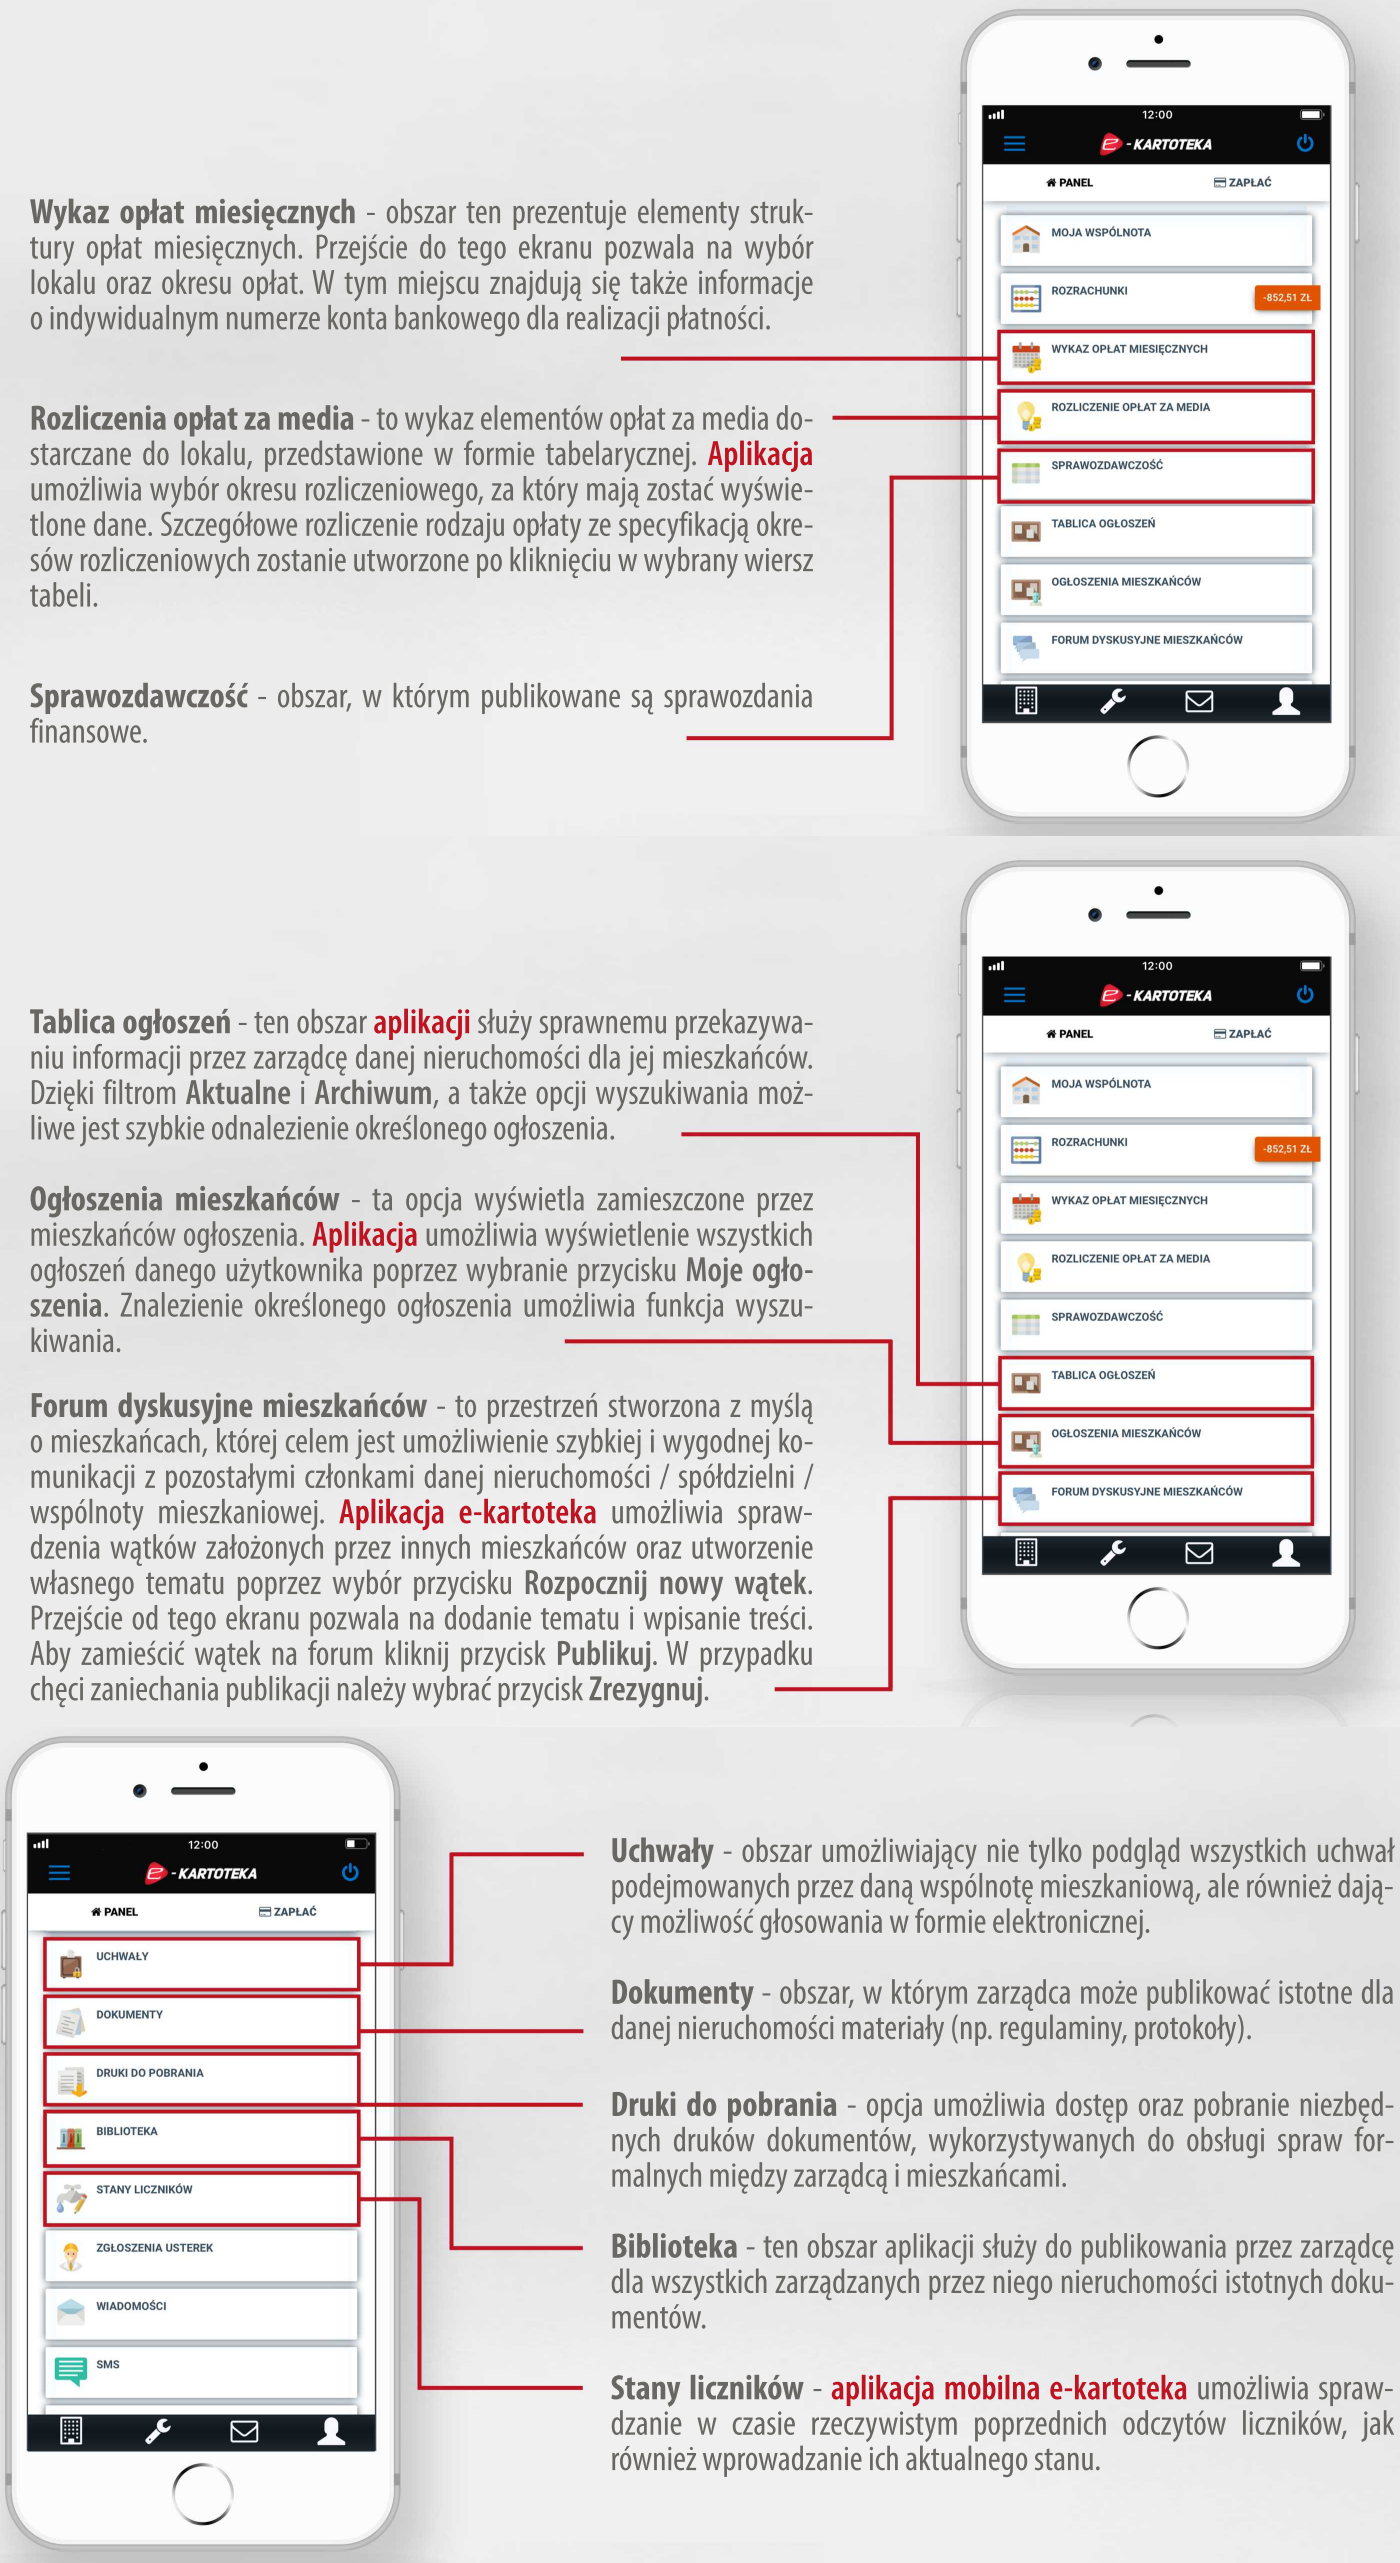
\includegraphics[width=0.63\linewidth]{rys01/kartoteka_manual}
    \caption{Opis głównych funkcji oferowanych w systemie ,,e-Kartoteka''~\cite{e-kartoteka_manual}}
    \label{fig:kartoteka_manual}
\end{figure}

Nowoczesne systemy eBOK eliminują konieczność bezpośredniego kontaktu, umożliwiając załatwienie większości spraw online, co zwiększa wygodę, oszczędność czasu oraz bezpieczeństwo transakcji i wymiany informacji. Jak widać mogą one różnić się między sobą zakresem oferowanych funkcji, skalowalnością oraz stopniem integracji z innymi systemami, jak np.\ narzędzia płatności online. Ich interfejsy mogą przyjąć postać aplikacji internetowych czy też mobilnych. Wybór odpowiedniej ścieżki implementacji zależy od potrzeb operacyjnych organizacji, liczby użytkowników oraz poziomu automatyzacji procesów. Wdrożenie eBOK-ów wymaga przemyślanego doboru technologii i architektury, co wiąże się z licznymi wyzwaniami. Opracowanie takich systemów stanowi dobrą okazję do rozwinięcia umiejętności programistycznych w obszarze automatyzacji procesów i zarządzania projektami IT. Dlatego też podczas formułowania tematu niniejszej pracy dyplomowej postanowiono tak go zadeklarować, by z jednej strony oferował walory poznawcze, z drugiej zaś był mocno osadzony w rzeczywistych realiach opisanej dziedziny. Jego finalna postać pozwala skupić się na rozwiązaniu problemu automatyzacji obsługi wspólnot mieszkaniowych oraz usprawnieniu komunikacji między mieszkańcami a administracją.

\section{Cel i zakres pracy}
Celem niniejszej pracy jest zaprojektowanie i wdrożenie aplikacji internetowej typu eBOK dla wspólnoty mieszkaniowej. Aplikacja ta powinna ułatwić zarządzania procesami związanymi z wewnętrzną komunikacją, płatnościami, zgłoszeniami technicznymi oraz dostępem do dokumentów. Dzięki niej zarówno mieszkańcy, jak i administratorzy uzyskają kompleksowe wsparcie podczas realizacji wielu codziennych zadań, co przyczynić się ma do lepszej samoorganizacji wspólnoty. Aplikacja tej nadano nazwę „Harmony Home Net”.

Zakres planowanych prac obejmuje pełny cykl rozwoju oprogramowania, od analizy potrzeb wspólnoty, poprzez projektowanie architektury systemu, aż po wdrożenie i przetestowanie gotowego rozwiązania. Analiza obejmie zarówno wymagania funkcjonalne, jak i niefunkcjonalne (bezpieczeństwo, wydajność oraz integracja z zewnętrznymi systemami). Przewiduje się iteracyjne testowanie oraz możliwość dalszego rozszerzania systemu o~nowe moduły.

Aplikacja będzie dostępna w przeglądarce internetowej i zoptymalizowana pod kątem dostępu z różnych urządzeń, w tym także w wersji desktopowej. Backend systemu zostanie stworzony w technologii Java i Spring Boot, co umożliwi budowę skalowalnych, bezpiecznych i łatwych w utrzymaniu aplikacji. Baza danych PostgreSQL będzie działać jako obraz Dockerowy, co zapewni izolację środowiska oraz ułatwi wdrażanie, zarządzanie i skalowanie aplikacji~\cite{EARTHLY}.

Frontend aplikacji zostanie zaprojektowany w języku TypeScript z wykorzystaniem frameworka Next.js, co pozwoli na stworzenie nowoczesnego, responsywnego interfejsu użytkownika, zapewniającego intuicyjną obsługę oraz szybkie działanie systemu.

\section{Układ pracy}
% tutaj opis zawartości kolejnych rozdziałów, można zredagować na końcu